\documentclass[12pt,a4paper]{article}
\usepackage[utf8]{inputenc}
\usepackage[spanish]{babel}
\usepackage{graphicx}
\usepackage{listings}
\usepackage{xcolor}
\usepackage{hyperref}
\usepackage{float}
\usepackage[margin=2.5cm]{geometry}
\usepackage{tocbibind} % Para incluir el índice en el índice
\usepackage{bookmark} % Mejora los bookmarks del PDF

% Configuración de colores para códigos
\definecolor{codegreen}{rgb}{0,0.6,0}
\definecolor{codegray}{rgb}{0.5,0.5,0.5}
\definecolor{codepurple}{rgb}{0.58,0,0.82}
\definecolor{backcolour}{rgb}{0.95,0.95,0.92}

\lstdefinestyle{mystyle}{
    backgroundcolor=\color{backcolour},   
    commentstyle=\color{codegreen},
    keywordstyle=\color{magenta},
    numberstyle=\tiny\color{codegray},
    stringstyle=\color{codepurple},
    basicstyle=\ttfamily\footnotesize,
    breakatwhitespace=false,         
    breaklines=true,                 
    captionpos=b,                    
    keepspaces=true,                 
    numbers=left,                    
    numbersep=5pt,                  
    showspaces=false,                
    showstringspaces=false,
    showtabs=false,                  
    tabsize=2
}

\lstset{style=mystyle}

\begin{document}
% Portada
\begin{titlepage}
    \centering
    \vspace*{1cm}
    
\includegraphics[width=0.8\linewidth]{espe.png}\\[0.5cm]
    
    \Large \textbf{Departamento de Ciencias de la Computación}\\
    \large \textbf{Universidad de las Fuerzas Armadas - ESPE}\\[0.5cm]
    
    \Huge \textbf{Práctica de Laboratorio No. 2}\\[0.3cm]
    \Large \textbf{Evaluación de herramientas de fuerza bruta en Kali Linux}\\[0.8cm]
    
    \textbf{Nombres:}\\
    Yeshua Amador Chiliquinga Amaya\\
    Cesar Ignacio Loor Mercado\\[0.3cm]
    
    \textbf{Carrera / Asignatura:} Ingeniería de Software / Ingeniería de Seguridad de Software\\
    \textbf{NRC:} 23358\\
    \textbf{Nombre del profesor:} Walter Fuertes, PhD\\[0.5cm]
    
    \textbf{Fecha de presentación:} 24 de mayo del 2025\\[1cm]    
    \vfill
\end{titlepage}
% Índice de contenido
\clearpage
\pdfbookmark{\contentsname}{toc} % Añade un bookmark al índice
\tableofcontents
\thispagestyle{empty}
\cleardoublepage
\setcounter{page}{1}

\section*{Objetivo de Aprendizaje}
\addcontentsline{toc}{section}{Objetivo de Aprendizaje}
Los estudiantes comprenderán el funcionamiento de las herramientas de fuerza bruta incluidas en Kali Linux al configurarlas y ejecutarlas en un entorno controlado utilizando un entorno virtual de red, evaluando su efectividad y limitaciones.

\section*{Bibliografía}
\addcontentsline{toc}{section}{Bibliografía}

\section*{Topología del Experimento}
\addcontentsline{toc}{section}{Topología del Experimento}

\begin{figure}[htbp]
    \centering
    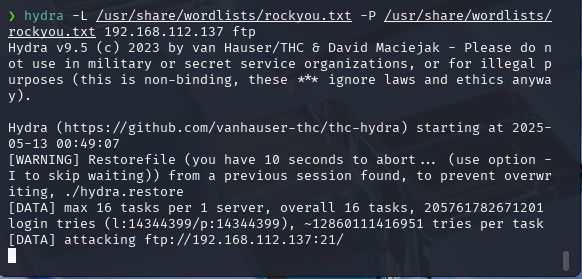
\includegraphics[width=0.8\textwidth]{hydra.png}
    \caption{Interfaz de Hydra}
    \label{fig:hydra}
\end{figure}

\begin{figure}[htbp]
    \centering
    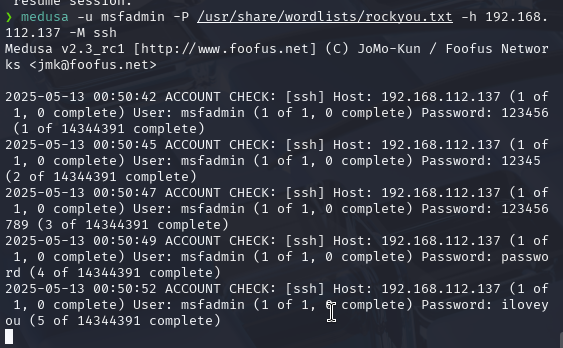
\includegraphics[width=0.8\textwidth]{medusa.png}
    \caption{Interfaz de Medusa}
    \label{fig:medusa}
\end{figure}

- Kali Linux.

    
- Una máquina objetivo con un sistema operativo como Metasploitable2, o un Servidor SSH o Web server.
    
- Documentos con usuarios y contraseñas para los ataques (Diccionarios).
    
- Lista de herramientas sugeridas: John the Ripper, Hydra, Medusa, Burp Suite, o Hashcat.


\section*{Marco Teórico}
\addcontentsline{toc}{section}{Marco Teórico}
Un ataque de fuerza bruta está dirigido contra la autenticación en el contexto de seguridad de la información. Vamos a desglosar los conceptos para entenderlo mejor:

\subsection{Autenticación vs Identificación}
\textbf{Identificación:} Proceso de declarar quién eres. \\
Ejemplo: Proporcionar un nombre de usuario o un identificador único, como un correo electrónico. \\
Pregunta clave: ¿Quién eres?

\textbf{Autenticación:} Proceso de verificar que eres quien dices ser. \\
Ejemplo: Proporcionar una contraseña, token, huella digital, o responder a un desafío basado en un factor de autenticación. \\
Pregunta clave: ¿Puedes demostrarlo?

\subsection*{El Ataque de Fuerza Bruta}
Un ataque de fuerza bruta intenta adivinar credenciales de autenticación, como contraseñas o claves. Se realiza probando sistemáticamente combinaciones de contraseñas o valores posibles hasta encontrar la correcta. \\
Propósito principal: Comprometer la autenticación (demostrar que se tienen las credenciales válidas). \\
No compromete directamente la identificación, porque esta etapa ya suele estar completa (el atacante usualmente conoce o asume un identificador, como un nombre de usuario).

\section{Desarrollo}
\subsection*{Ejecución de los Ataques utilizando John the Ripper: Crackear un hash de contraseña}
\begin{enumerate}
    \item Extraer hashes con \texttt{unshadow}:
    \begin{lstlisting}[language=bash]
unshadow /etc/passwd /etc/shadow > hashes.txt
    \end{lstlisting}
    \begin{verbatim}
        Using default input encoding: UTF-8
        Reading hashes.txt
        Press 'q' or Ctrl-C to abort, almost 
        any other key for status

        Loaded 4 password hashes with no different salts 
        (sha512crypt, crypt(3) $6$)
        Will run 4 OpenMP threads
        Proceeding with single, rules:Single
        0g 0:00:00:00 DONE (2025-05-20 16:35) 0g/s 1306Kp/s 
        1306Kc/s 1306KC/s 123..123
        Session completed
    \end{verbatim}
    
    \item Ejecutar John:
    \begin{lstlisting}[language=bash]
        john --wordlist=/usr/share/wordlists/rockyou.txt hashes.txt
    \end{lstlisting}
    \begin{verbatim}
        Using default input encoding: UTF-8
        Loaded 4 password hashes with no different salts 
        (sha512crypt, crypt(3) $6$ [SHA512 256/256 AVX2 4x])
        Will run 4 OpenMP threads
        Proceeding with wordlist:
        /usr/share/wordlists/rockyou.txt

        Press 'q' or Ctrl-C to abort, 
        almost any other key for status
        Loaded 4 password hashes with no different salts 
        (sha512crypt, crypt(3) $6$ [SHA512 256/256 AVX2 4x])
        Proceeding with wordlist:
        /usr/share/wordlists/rockyou.txt

        Press 'q' or Ctrl-C to abort, almost any other
         key for status
        Proceeding with incremental:ASCII
        Loaded 4 password hashes with no different salts 
        (sha512crypt, crypt(3) $6$ [SHA512 256/256 AVX2 4x])
        Proceeding with incremental:ASCII
        Press 'q' or Ctrl-C to abort, almost any other 
        key for status
    \end{verbatim}
\end{enumerate}

\subsection*{Crear el archivo \texttt{hashes.txt}}
El archivo \texttt{hashes.txt} es un archivo que contiene hashes de contraseñas, y es utilizado por herramientas como John the Ripper o Hashcat para crackear contraseñas. Para construirlo, necesitas extraer los hashes de contraseñas desde un sistema o crearlos manualmente.

\subsubsection*{Extraer hashes de un sistema Linux}
Si estás trabajando en un entorno controlado con un sistema Linux, los hashes de contraseñas se almacenan en los archivos \texttt{/etc/shadow} y \texttt{/etc/passwd}. Sigue estos pasos para extraerlos:

\begin{enumerate}
    \item \textbf{Acceso al sistema:} Asegúrate de tener permisos de superusuario (\texttt{root}) en el sistema donde deseas extraer los hashes.
    \item \textbf{Combinar \texttt{passwd} y \texttt{shadow}:} Utiliza el comando \texttt{unshadow} para combinar los archivos \texttt{/etc/passwd} y \texttt{/etc/shadow} en un formato que pueda usar John the Ripper.
    \begin{lstlisting}[language=bash,breaklines=true]
unshadow /etc/passwd /etc/shadow > hashes.txt
    \end{lstlisting}
    \begin{verbatim}
Using default input encoding: UTF-8
Reading hashes.txt
Press 'q' or Ctrl-C to abort, almost any other key for status

Loaded 4 password hashes with no different salts 
(sha512crypt, crypt(3) $6$)
Will run 4 OpenMP threads
Proceeding with single, rules:Single
0g 0:00:00:00 DONE (2025-05-20 16:35) 0g/s 1306Kp/s 
1306Kc/s 1306KC/s 123..123
Session completed
    \end{verbatim}
    Esto generará un archivo \texttt{hashes.txt} que contiene las credenciales (en formato hash) de las cuentas locales.
\end{enumerate}

\subsection*{¿Qué es el archivo \texttt{rockyou.txt}?}
El archivo \texttt{rockyou.txt} es una lista de contraseñas comúnmente utilizada en pruebas de penetración y auditorías de seguridad. Contiene millones de contraseñas filtradas, ordenadas por popularidad, que provienen de una brecha masiva de datos del sitio de redes sociales RockYou en 2009. Es ampliamente empleado para realizar ataques de fuerza bruta y pruebas de diccionario en herramientas como Hydra, John the Ripper, Medusa, y Hashcat.

\subsubsection*{Ubicación del archivo en Kali Linux}
El archivo \texttt{rockyou.txt} está preinstalado en Kali Linux, pero está comprimido por defecto para ahorrar espacio en disco. Puedes encontrarlo en la siguiente ruta:
\begin{verbatim}
/usr/share/wordlists/rockyou.txt.gz
\end{verbatim}

\subsubsection*{Cómo descomprimir el archivo \texttt{rockyou.txt}}
Para usar este archivo, primero necesitas descomprimirlo:
\begin{lstlisting}[language=bash]
gunzip /usr/share/wordlists/rockyou.txt.gz
\end{lstlisting}
\begin{verbatim}
rockyou.txt.gz: 52.5% -- replaced with rockyou.txt
\end{verbatim}
Ahora el archivo estará disponible en:
\begin{verbatim}
/usr/share/wordlists/rockyou.txt
\end{verbatim}

\begin{figure}[htbp]
    \centering
    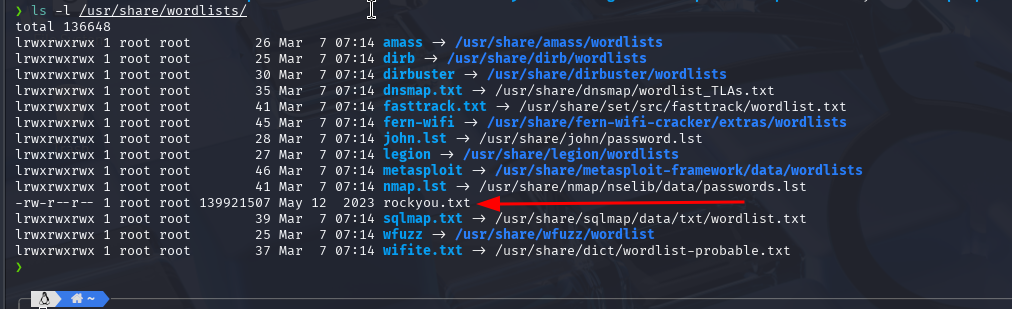
\includegraphics[width=0.8\textwidth]{rockyou.png}
    \caption{Ubicación del archivo rockyou.txt en Kali Linux}
    \label{fig:rockyou}
\end{figure}

\section*{Resultados}
\addcontentsline{toc}{section}{Resultados}
Cada grupo debe registrar:

    
- Configuración del entorno.
    
- Comandos utilizados.
    
- Resultados obtenidos (éxito/fallo, tiempo, etc.).
    
- Limitaciones observadas en la herramienta.


\section*{Plenaria de Análisis y Discusión}
Cada grupo presenta sus hallazgos al resto de la clase:

    
- Comparar la efectividad de las herramientas.
    
- Identificar estrategias para mitigar ataques de fuerza bruta.


\section*{Conclusiones}
\addcontentsline{toc}{section}{Conclusiones}
Un ataque de fuerza bruta se dirige contra la autenticación, ya que su objetivo es adivinar contraseñas, claves o factores de acceso relacionados con este proceso. Sin embargo, puede complementarse con ataques contra la identificación, como la enumeración de usuarios, para obtener más información sobre posibles objetivos.

La efectividad de los ataques de fuerza bruta depende de varios factores, como la complejidad de las contraseñas, las limitaciones impuestas por el sistema objetivo (por ejemplo, bloqueos tras múltiples intentos fallidos), y la calidad del diccionario utilizado.

En la práctica, los ataques tuvieron mayor éxito contra configuraciones inseguras o contraseñas débiles, resaltando la importancia de implementar contraseñas fuertes y mecanismos de defensa como límites de intentos y autenticación multifactor.

Los resultados demuestran que, aunque efectivos en ciertos escenarios, los ataques de fuerza bruta son altamente dependientes del contexto y consumen tiempo y recursos, especialmente contra sistemas bien configurados.

\section*{Referencias}

    
- Kali Linux Documentation. (2024). Tools Listing. Recuperado de \url{https://www.kali.org/tools/}
    
- Offensive Security. (2024). Metasploitable 2. Recuperado de \url{https://sourceforge.net/projects/metasploitable/}
    
- Bishop, M. (2019). Introduction to Computer Security. Boston, MA: Addison-Wesley.
    
- Katz, J., \& Lindell, Y. (2020). Introduction to Modern Cryptography. Chapman \& Hall/CRC.
    
- W Fuertes, M Macas, Ciberseguridad: Del ciber-crimen a los ataques ciber-físicos, Comité Editorial de la ESPE, Sangolquí, Ecuador. ISBN: 978-9942-765-88-8 1, 190


\end{document}